\DiaryEntry{Fundamental Theorem of Calculus}{2018-09-05}{Maths}


The fundamental theorem of calculus relates differentiation and integration, showing that these two operations are essentially inverses of one another.

\subsection{Geometric Interpretation / Intuition}

Consider a continuous function $f(x)$, with "area function" $F(x)$ which represents the area under the function between $0$ and $x$. This is in fact the definite integral $F(x) = \int_0^x f(x) dx$. We are interested in the relation between $f(x)$ and $F(x)$. To this end consider the area change $F(x+\Delta x) - F(x)$. Looking at the Figure below, we can approximate this difference as follows

\bee
F(x+\Delta x) - F(x) \approx f(x) \Delta x
\eee

We can rearrange this to

\bee
f(x) \approx \frac{F(x+\Delta x) - F(x)}{\Delta x}
\eee

and in the limit of very small $\Delta x$ we obtain the exact expression

\bee
f(x) = \lim_{\Delta x \rightarrow 0} \frac{F(x+\Delta x) - F(x)}{\Delta x}
\eee

This shows that the area function $F(x)$ is the function which differentiated becomes $f(x)$; i.e. the anti-derivative of $f(x)$.

\begin{figure}[H]
	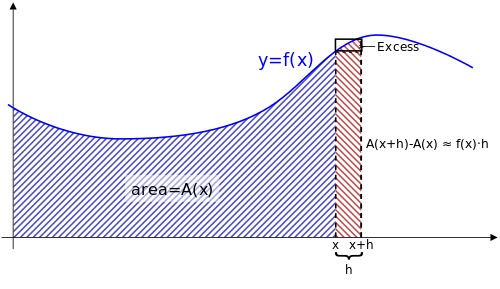
\includegraphics[scale=0.65]{images/fund_theorem_calculus.png}
\end{figure}


\subsection{Formal Statements}

There are actually two parts: The first part deals with the derivative of an anti-derivative, while the second part deals with the relationship between anti-derivatives and definite integrals. 

\paragraph{First Part.} Let $f$ be a continuous real-valued function defined on a closed interval $[a, b]$. Let $F$ be the function defined, for all $x$ in $[a, b]$, by

\bee
F(x)=\int_{a}^{x} f(t) dt
\eee

Then, $F$ is uniformly continuous on $[a, b]$, differentiable on the open interval $(a, b)$, and

\bee
F'(x) = f(x)
\eee

for all $x$ in $(a, b)$.

\paragraph{Corollary.} If $f$ is a real-valued continuous function on $[ a , b ]$ and $F$ is an anti-derivative of $f$ in $[ a , b ]$ [a,b] then

\bee
\int _{a}^{b} f(t) dt = F(b)-F(a)
\eee

The corollary assumes continuity on the whole interval. 

\paragraph{Second Part.} Let $f$ be a real-valued function on a closed interval $[a,b]$ and $F$ an anti-derivative of $f$ in $[a,b]$, 

\bee
F'(x)=f(x)
\eee

If $f$ is Riemann integrable on $[a,b]$ then

\bee
\int_{a}^{b}f(x) dx = F(b)-F(a)
\eee

The second part is somewhat stronger than the corollary because it does not assume that $f$ is continuous.


\subsection{Proofs}

\paragraph{First Part.} For a given $f(t)$, define the function $F(x)$ as

\bee
F(x)=\int_{a}^{x}f(t) dt
\eee

For any two numbers $x_1$ and $x_1 + \Delta x$ in $[a, b]$, we have

\bee
F(x_1)=\int_{a}^{x_{1}} f(t) dt, \qquad F(x_{1}+\Delta x) = \int_{a}^{x_{1}+\Delta x}f(t)dt
\eee

Subtracting these two expressions from each other yields

\be\label{eq:2018-09-05:1}
F(x_{1}+\Delta x) - F(x_1) = \int_{a}^{x_{1}+\Delta x}f(t)dt - \int_{a}^{x_{1}}f(t)dt = \int_{x_1}^{x_{1}+\Delta x}f(t)dt
\ee

According to the mean value theorem for integration, there exists a real number $c \in [x_{1},x_{1}+\Delta x]$ such that

\bee
\int _{x_{1}}^{x_{1}+\Delta x}f(t)\,dt=f(c)\cdot \Delta x
\eee

Note that $c$ will depend on $f$, $x_1$, and $\Delta x$ but will always be in the interval $[x_{1},x_{1}+\Delta x]$.

Inserting into \eqref{eq:2018-09-05:1} and dividing by $\Delta x$, we obtain

\bee
f(c) = \frac{F(x_{1}+\Delta x) - F(x_1)}{\Delta x}
\eee

Taking the limit $\Delta x \rightarrow 0$ on both sides we obtain

\bee
\lim_{\Delta x \rightarrow 0} f(c) = \lim_{\Delta x \rightarrow 0} \frac{F(x_{1}+\Delta x) - F(x_1)}{\Delta x}
\eee

The left hand side becomes $f(x_1)$ (remember that $c$ is in the interval $[x_{1},x_{1}+\Delta x]$) and we are "squeezing" the interval; the right hand side becomes $F'(x_1)$. Combining, we therefore have

\bee
F'(x) = f(x) \qed
\eee

\paragraph{Corollary.} Suppose $F$ is an anti-derivative of $f$, with $f$ continuous on $[a, b]$. Let

\bee
G(x)=\int_{a}^{x}f(t) dt
\eee

By the first part of the theorem, we know $G$ is also an anti-derivative of $f$. Since $F' - G' = 0$ (the mean value theorem - really needed?) implies that $F - G$ is a constant function, i. e. there is a number $c$ such that $G(x) = F(x) + c$, for all $x$ in $[a, b]$. Letting $x = a$, we have

\bee
F(a)+c = G(a) = \int_{a}^{a}f(t) dt = 0
\eee

which means $c = - F(a)$. In other words, $G(x) = F(x) - F(a)$, and so

\bee
\int_{a}^{b}f(x) dx = G(b) = F(b)-F(a) \qed
\eee

\paragraph{Second part.} Short sketch only (the full version is \href{https://en.wikipedia.org/wiki/Fundamental_theorem_of_calculus}{here}): Let there be numbers $x_1,\ldots,x_n$ such that

\bee
a=x_{0}<x_{1}<x_{2}<\cdots <x_{n-1}<x_{n}=b
\eee

With some steps omitted, we can write

\bee
F(b)-F(a) = \sum_{i=1}^{n} [f(c_{i})(\Delta x_{i})]
\eee

Letting $\Delta x_i$ go to zero (which implies an the number of points to go to infinity), we have

\bee
F(b)-F(a) = \int_{a}^{b}f(x) dx \qed
\eee


%%% Local Variables:
%%% mode: latex
%%% TeX-master: "journal"
%%% End:
